% ****** Start of file apssamp.tex ******
%
%   This file is part of the APS files in the REVTeX 4.1 distribution.
%   Version 4.1r of REVTeX, August 2010
%
%   Copyright (c) 2009, 2010 The American Physical Society.
%
%   See the REVTeX 4 README file for restrictions and more information.
%
% TeX'ing this file requires that you have AMS-LaTeX 2.0 installed
% as well as the rest of the prerequisites for REVTeX 4.1
%
% See the REVTeX 4 README file
% It also requires running BibTeX. The commands are as follows:
%
%  1)  latex apssamp.tex
%  2)  bibtex apssamp
%  3)  latex apssamp.tex
%  4)  latex apssamp.tex
%
\documentclass[
reprint,
 amsmath,amssymb,
 aps,
 prl
]{revtex4-1}

\newcommand{\partDeriv}[2]{\frac{\partial #1}{\partial #2}}
\DeclareMathOperator\erf{erf}

\usepackage{graphicx}% Include figure files
\usepackage{dcolumn}% Align table columns on decimal point
\usepackage{bm}% bold math
\usepackage{hyperref}


\begin{document}

\title{On The Diffusion of Sticky Particles in 1-D}

\author{Joshua DM Hellier}
 \email{J.D.M.Hellier@sms.ed.ac.uk}
\author{Graeme J Ackland}
 \email{G.J.Ackland@ed.ac.uk}
\affiliation{
 SUPA, School of Physics and Astronomy, University of Edinburgh, Mayfield Road, Edinburgh EH9 3JZ, United Kingdom
}

\date{\today}% It is always \today, today,
             %  but any date may be explicitly specified

\begin{abstract}
The 1D Ising model is the simplest Hamiltonian-based model in
statistical mechanics. The simplest interacting particle process is
the Symmetric Exclusion Process (SEP), a 1D lattice gas of particles
that hop symmetrically and cannot overlap.  Combining the two gives a
model for sticky particle diffusion, SPM, which is described here.
SPM dynamics are based on SEP with short-range interactions, allowing
flow due to non-equilibrium boundary conditions.  We prove that SPM is
also a detailed-balance respecting, particle-conserving, Monte Carlo
description of the Ising model.  Neither the Ising model nor SEP have
a phase transition in 1D, but the SPM exhibits a non-equilibrium
transition.  This transition is from normal diffusion to a state with close-to-zero flow,
breaking into a two-phase mixture.  We present a fully
non-linear, analytic, mean-field solution, which has a crossover from
a positive to a negative diffusion constant coincident with the full SPM 
transition. Thus, the mean field theory successfully predicts its own demise.
The simplicity of the model suggests a wide range of possible
applications.


\end{abstract}

%\keywords{Suggested keywords}%Use showkeys class option if keyword
                              %display desired
\maketitle




Lattice gases are a ubiquitous tool for modeling complex systems from
biology to traffic~\cite{1742-5468-2011-07-P07007, Mobilia2007,
  tegner2015high, zhu2012atomic, DealGrove1965, MottCabrera1949,
  Buzzaccaro2007}.  Analytically solvable cases involve
non-interacting or excluding particles, but in any real system of
interest, the moving objects interact. Many models tackle the situation
where the diffusing objects interact with an external field or the
substrate~\cite{ladd1988application, liggett1985interacting,
  BenNaim1999, Shandarin1989, Frachebourg1999, Frachebourg2000}, and
non-trivial flow is induced by these non-equilibrium interactions.  

For many applications, one is interested in a system where the only
non-equilibrium feature is a driving force applied at the boundaries,
such as a chemical potential difference, while far from the
boundaries the system is free to self-organize due to interactions between the particles.
Surprisingly, there are few such models in the literature.
One reason for this is
that the interactions introduce nonlinearities in analytical models,
which makes them challenging to solve, at least outside of limits in
which they can be linearized. This is unfortunate because it is
precisely these nonlinearities which introduce interesting behaviors
such as discontinuities at the oxide-metal interface or diffusion
instability~\cite{Obukhovsky2017,Gorokhova2010}.

Here we investigate a simple one-dimensional flow model with
interparticle interactions, the ``Sticky Particle Model'' (SPM),
specified in the top left inset of Fig.~\ref{fig:lambdaScans}.


There are many examples of models of driven-dissipative dynamics. It
is sometimes assumed that locally non-equilibrium dynamics are
required to model complex flows. The novel feature of SPM is that it
has locally homogeneous equilibrium dynamics (i.e. it obeys detailed balance, has no
external field, and has no interaction with the substrate). Nevertheless, it exhibits a
nonequilibrium phase transformation from a homogeneous, diffusing
phase to a jammed structure.  We thereby demonstrate that while local
dissipation or substrate interactions can cause non-diffusive flow,
they are not a necessary requirement.


\iffalse
\begin{figure}
\vspace{1em}
    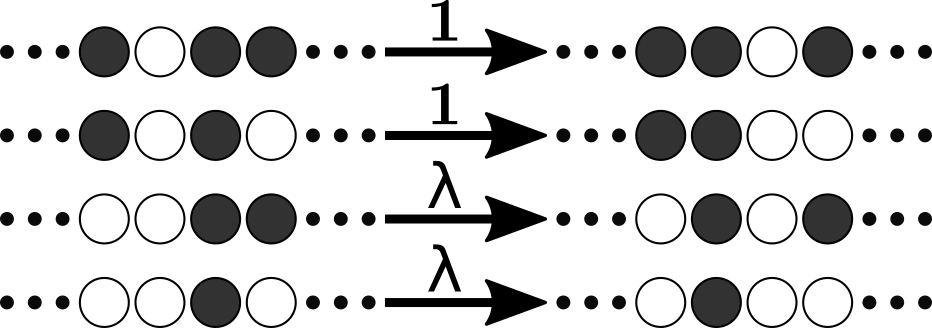
\includegraphics[width=\linewidth]{newRates}
\caption{\label{fig:rates} White circles indicate particles, dark circles indicate empty sites (vacancies). Particles randomly move into adjacent vacancies with rate $1$ (having rescaled time for notational convenience), unless there is a
particle behind the position they're moving from, in which case they move with rate $\lambda$; the state of the site next to the position the particle is moving into is irrelevant.
Particles also move to the left, with rates such that the whole model is totally symmetric.}
    \vspace{-3em}
\end{figure}
\fi

\begin{figure}[h!]
\setbox1=\hbox{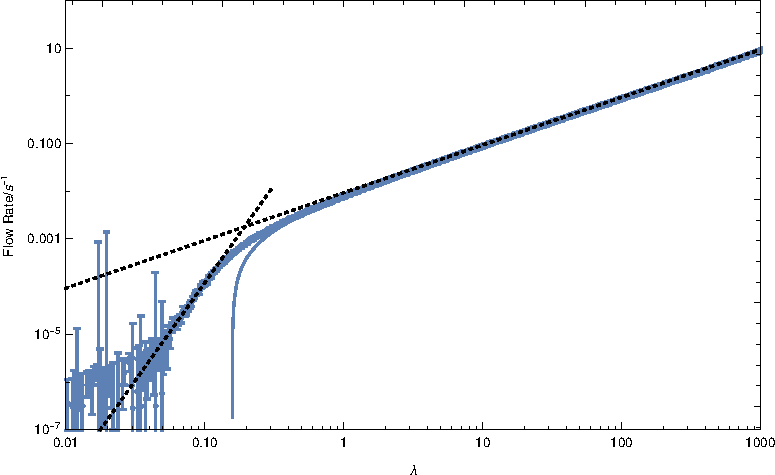
\includegraphics[width=\linewidth]{logFlowRates}}
  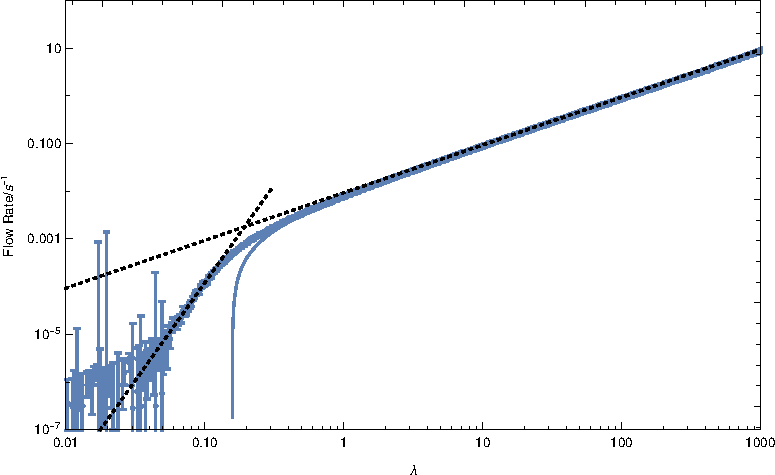
\includegraphics[width=\linewidth]{logFlowRates}\llap{\makebox[0.525\linewidth][l]{\raisebox{0.6cm}{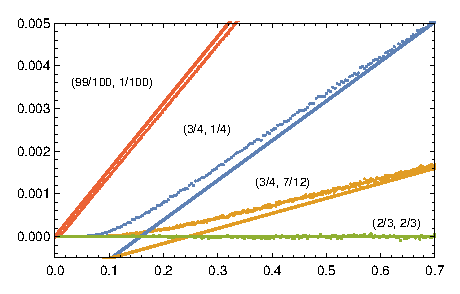
\includegraphics[width=0.475\linewidth]{linearFlowRates}}}}\llap{\makebox[0.9\linewidth][l]{\raisebox{3.75cm}{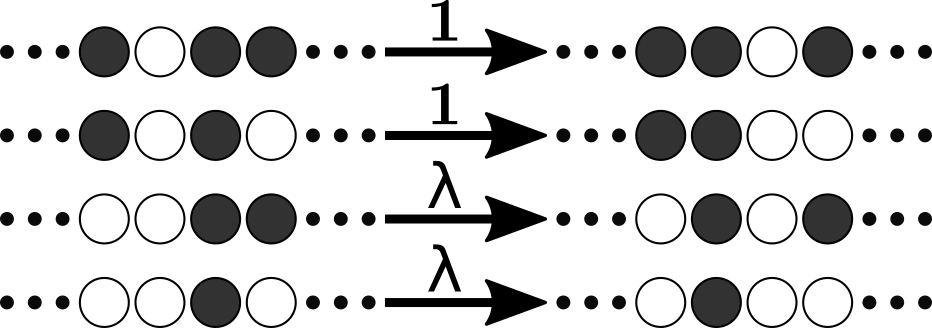
\includegraphics[width=0.45\linewidth]{newRates}}}}
    \vspace{-1em}
\vspace{1em}
\caption{\label{fig:lambdaScans} \textbf{Top left:} SPM dynamics:
  White circles indicate particles, dark circles indicate empty sites
  (vacancies). Particles randomly move into adjacent vacancies with
  rate $1$, unless there is an adjacent particle, in which case they
  move with rate $\lambda$; the state of the site beyond the new
  position is irrelevant.  Particles can move left or right, such that
  the whole model is totally symmetric.\\ \textbf{Bottom right:} Mean
  flow rate as a function of $\lambda$ with fixed boundary densities
  $(\rho_0, \rho_L)$ as labeled in the plot.  The MFT predictions are
  indicated by the solid line.  Each data point is derived from
  systems of length $64$ (length $32$, $128$ and $256$ give similar
  results), each using over $10^8$ Gillespie steps: $4\times10^5$ for
  equilibration, followed by $10^4$ measurement runs of $10^3$ steps
  interspersed with $16000$ decorrelation steps.  The $10^4$
  uncorrelated samples allow us to measure accurate flow rates and
  densities and the statistical distributions of both quantities; flow
  moments and the density data are given as supplementary
  materials.\\ \textbf{Main figure:} Log-log plot of the $\left(
  \frac{3}{4} , \frac{1}{4} \right)$ data, extended over many orders
  of magnitude of $\lambda$.  The dashed lines represent asymptotic
  power-laws; the higher-$\lambda$ one matches the mean-field,
  diffusion-limit prediction (solid line) with flow~$\propto \lambda^1$, whilst the
  lower-$\lambda$ one - fitted in the range $0.04 \le \lambda \le 0.1$
  - shows critically-slowed flow with flow~$\propto \lambda^4$.
\vspace{1em}}
\end{figure}

The SPM is based upon the symmetric exclusion
process~\cite{sugden2007dynamically, Kollmann2003, Lin2005, Hegde2014,
  Krapivsky2014, Imamura2017}, augmented by an interaction rule which specifies that
adjacent particles separate with rate $\lambda$ instead of their
normal hopping rate, $1$. 
The quantity $\lambda$
parametrizes the ``stickiness'' of the particles; when $\lambda>1$,
there is a tendency for particles to repel, whilst $\lambda < 1$
represents attraction.  We prove in the supplementary materials that
the rates specified in Fig.~\ref{fig:lambdaScans} obey detailed
balance, with a Hamiltonian isomorphic to the Ising model.

%It is worth noting that the rates specified in Fig.~\ref{fig:rates} obey detailed balance,  %cite supplementary materials
%with an energy proportional to the number of particle-particle adjacencies
%in the system. It seems that space of highly-local exclusion models is so tightly constrained in one-dimension that there is no option but to comply with the detailed balance condition.
One might contrast this approach (making a simple microscopic model
and trying to learn from it about large-scale interface growth) with
continuum approaches such as the KPZ
equation~\cite{PhysRevLett.56.889, PhysRevA.38.4271, Sasamoto2010}
where one analyses the extreme large-scale dynamics using universality
classes.  The particle-conserving dynamics of SPM are like
those used to analyze the equilibrium Ising model by
Kawasaki~\cite{PhysRev.145.224}.  SPM can be viewed as a simplified KLS
model~\cite{Katz1984, Zia2010, Kafri2003} in 1-dimension without an
applied field.  The KLS model 
has very interesting behaviour attributed to the applied field; however, 
we shall show that our simplified, symmetric model also
exhibits complex unexpected behavior when driven by a chemical
potential difference at the boundary. 


Numerical simulation reveals 
the wide range of the SPM
behaviors, such as those shown in Fig.~\ref{fig:flowPatterns}. We will
discuss these numerical results in more detail later, but first let us
analyze the model analytically.  Because of the
interactions, the types of methods used for the full analytic
solution of SEP cannot be applied; thus we pursue a
mean-field theory approximation.  

Let the spacing between lattice sites be $a$, let $\tau_0$ be the
free-particle hopping timescale, and the time-averaged (or
ensemble-averaged, assuming ergodicity) occupation probability of the
$i^{\mathrm{th}}$ lattice site be $\rho_i$.  We introduce $\zeta = 1 -
\lambda $ here for convenience: high $\zeta$ implies sticky particles,
negative $\zeta$ implies repulsion.  It is demonstrated in the
supplementary materials that, in mean-field approximation regime,
% maybe derive in appendix
\begin{align}
\begin{split}
 \tau_0 \partDeriv{\rho_i}{t} = &\left( 1-\rho_i \right) \left[ \left(1-\zeta\rho_{i-2} \right) \rho_{i-1} + \left(1-\zeta\rho_{i+2} \right) \rho_{i+1} \right] \\
 &- \rho_i \left[ 2 \zeta \rho_{i-1} \rho_{i+1}  - (3-\zeta)\left(\rho_{i-1} + \rho_{i+1}\right) + 2 \right].
 \end{split}
 \end{align}
Switching to the continuum limit by taking $a\rightarrow 0$, and neglecting $\mathcal{O}(a^4)$ terms, we may re-express this as a conserved flow $J$ as follows:
\begin{align}
 \partDeriv{\rho}{t} &= - \partDeriv{J}{x}, \\
 J &= -  D(\rho) \partDeriv{\rho}{x}, \\
 D(\rho) &= \frac{a^2}{\tau_0} \left[1 - \zeta \rho\left(4-3\rho\right) \right]. \label{eq:diffCoeff} 
\end{align}
Thus, the MFT says that the particles should diffuse with a diffusion coefficient $D(\rho)$ which depends upon the local density, and exhibits an unexpected symmetry about $\rho=\frac{2}{3}$.

In order to understand the implications of the MFT, let us consider
some limits. As $\zeta \rightarrow 0$ (i.e. as the model becomes a
simple exclusion model), $D \rightarrow \frac{a^2}{\tau_0}$. Likewise,
in the dilute limit $\rho \rightarrow 0$, $D \rightarrow \frac{
  a^2}{\tau_0}$, reflecting the fact that the interactions become
irrelevant as particles never meet.  Conversely, in the full limit
$\rho \rightarrow 1$, $D \rightarrow \frac{\lambda a^2}{\tau_0}$;
 we now have a dilute gas of vacancies, which hop with rate
$\frac{\lambda}{\tau_0}$.  One may observe that
equation~\ref{eq:diffCoeff} has a symmetry under $\rho \mapsto
\frac{4}{3} - \rho$; thus, the dynamics should be symmetric under a
density profile reflection around $\rho = \frac{2}{3}$. This is where
$D$ always attains its extremal value, $ \frac{a^2}{\tau_0}\left[1 -
  \frac{4}{3}\zeta\right]$; hence for $\zeta>3/4$ the MFT diffusion
coefficient becomes negative in regions with $\frac{2}{3} -
\frac{\sqrt{\zeta\left(4\zeta - 3\right)}}{3\zeta} < \rho <
\frac{2}{3} + \frac{\sqrt{\zeta\left(4\zeta - 3\right)}}{3\zeta}$.
Finally,  solutions to the continuum MFT
containing domains with a negative diffusion coefficient are linearly
unstable; thus, if $D_{MFT}(\rho)<0$, $\rho$ itself is unstable with
respect to either of the two densities for which $D(\rho)\sim
0$ (see SM for proof). Instead of observing ``backwards diffusion'' we would see an
extremely slow flow or no flow at all. The MFT implies that the
transition to this critically slowly-flowing regime happens suddenly,
like a phase transition: this can be checked with numerics.

It is possible to solve the continuum MFT in a steady state on a finite domain, say $x\in(0, L)$. The continuity equation implies that $J(x)=J_0=\mathrm{const.}$, and by integrating both sides of this equation with respect to $x$ we find that
\begin{equation}
 J(x) = (x-x_0)J_0 = -\frac{a^2}{\tau_0} \rho \left[1+\zeta \rho\left(\rho-2\right)\right], \label{cubic}
\end{equation}
a cubic equation which can be solved to give $\rho(x)$
with appropriately chosen real constant $x_0$. If we impose Dirichlet boundary conditions on this system, say $\rho(0)=\rho_0$ and $\rho(L)=\rho_L$, we find that
\begin{equation}
\label{eq:boundedFlow}
 J_0 = \frac{a^2}{L \tau_0} \left[ \rho_0 - \rho_L + \zeta \left( \rho_0\left[\rho_0^2-2\right] - \rho_L\left[\rho_L^2-2\right] \right) \right].
\end{equation}
We may consider applying small concentration gradients across a domain by setting $\rho_0 = \rho_M + \frac{1}{2}\delta\rho$ and $\rho_L = \rho_M - \frac{1}{2}\delta\rho$. Doing so, we find that the effective diffusion coefficient of the domain
$D_\mathrm{Eff}=L \partDeriv{J}{\delta\rho}\big|_{\delta\rho=0}$ obeys
\begin{equation}
\label{eq:MFTflow}
 D_\mathrm{Eff} = \frac{a^2}{ \tau_0} \left[ 1 - \zeta\rho_M(4-3\rho_M) \right],
\end{equation}
which implies the same symmetry about $\rho=\frac{2}{3}$ and negative
flow region as Eq.~\ref{eq:diffCoeff}


We implemented the SPM numerically using the  Gillespie algorithm~\cite{Gillespie1977, Bortz1975, Prados1997} implemented in the \texttt{KMCLib}~\cite{leetmaa2014kmclib}  Kinetic Monte Carlo 
package. The codes are publicly available~\cite{jHellGitRepo}.
%\texttt{KMCLib} has the advantage that it is python-wrapped \texttt{C++}, and thus quite easy to use whilst at the same time being quite computationally efficient; thus it was fairly easy for us to carry out large numbers
%of differently-parametrised serial \texttt{KMCLib} jobs on the \texttt{Eddie3} computing cluster here at Edinburgh. As we have MFT predictions about flow in a bounded domain, we can simulate that situation using KMC.
% In the bulk, the transition rates are simply those described in Fig.~\ref{fig:lambdaScans}. 
With periodic boundary conditions, we recover the fixed magnetization Ising Model, as expected.

To investigate flow, we set up a chemical potential difference across
the system by defining the boundaries. We use two boundary-layer
lattice sites which switch between being full and empty such that
their time-averaged occupation matches the desired concentration;
there are then chances for particles to appear and disappear at these
boundary layers, as well as migrate into the main part of the
system. These boundary conditions reproduce the effect of having
particle reservoirs attached to the edges of the domain, which we
verified by inspecting the time-averaged occupations of sites near the
boundary.

We have used the setup above to  explore three scenarios, discussed in
the following sections. In each of these we refer to a boundary
condition configuration by $(\rho_0, \rho_L)$, with $\rho_0$ and
$\rho_L$ being the boundary densities at opposite ends of the system
of length $L$.  We measure overall particle flow rate from the number
of particles entering and leaving, and maintain a histogram of the
distribution of the number of particles in the system.  Our initial
configurations have randomly distributed particles with density
$\frac{1}{2}(\rho_0 + \rho_L)$, and we then run the system for a
sufficient number of equilibration steps to destroy any initial
transients.

The MFT suggested that a transition from a steady flow regime to a
critically slow flow regime might occur as the stickiness varies.  We
test for this by measuring the particle density as well as the mean,
variance and skewness of the flow rate as a function of
$\lambda$ for fixed $(\rho_0, \rho_L)$. If such a transition does
indeed occur, we should expect to see something interesting happen as
$\lambda$ passes through the transition point. 

\iffalse
\begin{figure*}[h!]
\vspace{1em}
\caption{\label{fig:lambdaScans} Descriptive statistics of flow rates and average overall densities observed when varying $\lambda$ with fixed boundary densities $(\rho_0, \rho_L)$; data series are labelled in the plot.
In the case of the mean flow we have an MFT prediction, indicated by the solid line.
In each case we used systems of length $64$ (length $32$ gives similar results),
running them for $400000$ Gillispie steps for equilibration followed by $10000$ measurement runs of $1000$ steps interspersed with relaxation runs of $16000$
steps. This way we could gather statistics about flow rates and densities in a well-equilibrated system. Specifically, we generate a pool of $10000$ samples of flow rate and density,
from which we can calculate estimates of the descriptive statistics of both quantities.}
\begin{center}
 \begin{tabular}{c|c}
    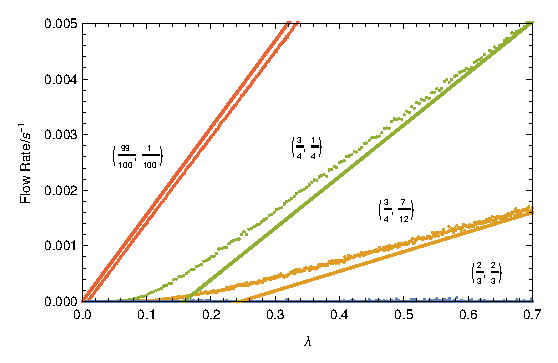
\includegraphics[width=0.5\linewidth]{../tex-src/lambdaScan/newFlowMean} & 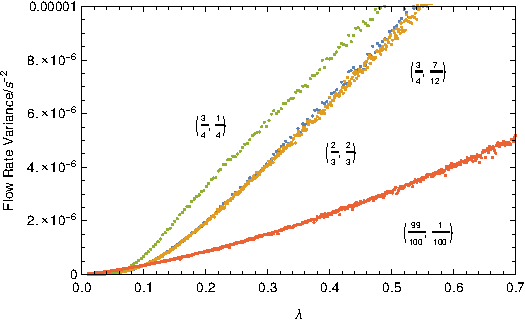
\includegraphics[width=0.5\linewidth]{../tex-src/lambdaScan/newFlowVar} \\
    \hline
    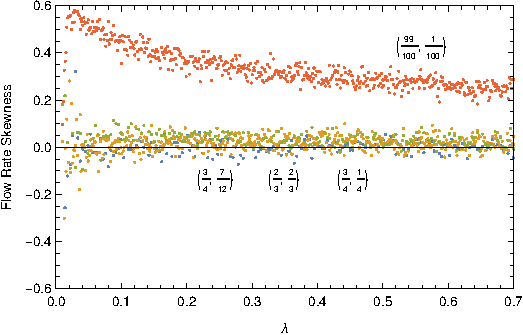
\includegraphics[width=0.5\linewidth]{../tex-src/lambdaScan/newFlowSkew} & 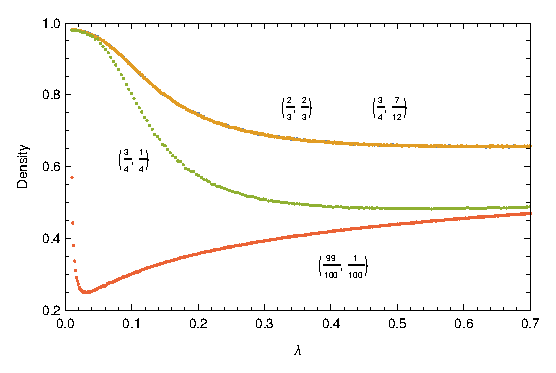
\includegraphics[width=0.5\linewidth]{../tex-src/lambdaScan/newDens} \\
    \end{tabular}
\end{center}
    \vspace{-0em}
\end{figure*}
\fi


Fig.~\ref{fig:lambdaScans} shows a log-log plot of flow rate over a
large range of $\lambda$ for fixed boundary conditions.  The inset
shows the effect of boundary conditions.  The equivalent MFT results
are calculated using Eq.~\ref{eq:boundedFlow}, which is predicted to break down when  $\lambda\sim\frac{1}{4}$,
below which the MFT
flow becomes negative.  The simulated SPM flow does continue, at a much reduced 
rate and
with different power-law behavior from particle diffusion.  This
different flow behavior defines the SPM transition.
For low-stickiness ($\lambda>\frac{1}{4}$) the
MFT is in very good agreement with the simulations, and this continues
for repulsive $\lambda>>1$, where the mean flow rate varies linearly
with $\lambda$.

For very high stickiness ($\lambda<0.04$), convergence is very slow,
hence the large standard errors. However, there is a regime when $0.04
\le \lambda \le 0.1$ where the mean flow displays clear
$\mathcal{O}(\lambda^{4})$ power-law behaviour.  Defining the SPM
transition by where the power laws cross at $\lambda = 0.194$, gives
good agreement with the MFT transition to negative flow.  The key
point here is that as that as we pass from high-$\lambda$ to
low-$\lambda$, the scaling in $\lambda$ does change, which suggests to
us that the mechanism by which material is transferred through the
medium changes from the standard diffusive one (which is
well-described by the MFT) to something different, which to our
knowledge has not been previously observed.  In this region the MFT
assumption of $\rho\sim\rho_M = \frac{1}{2}(\rho_0 + \rho_L)$ has broken down, and the number of
particles in the system increases (see SM).  We can interpret the
critically slow flow as being due to rare-event fluctuations in an
otherwise full region.
%However, one of the key predictions of the MFT - that a sharp transition to a no-flow regime occurs when $\lambda$ becomes small enough (at least for 3 of the 4 sets of
%boundary conditions we investigated here) - is not realized in our simulations. Indeed what seems to be happening is that the sharp transition has been smoothed out, as we
%do not see any peaks or jumps in the flow rate variance or skewness (which we would expect to see if there was a transition). We suspect that this discrepancy is due to nontrivial correlations emerging between the particles, which the MFT
%does not take account of. Alternatively, it could be that the continuum assumption is failing due to the finite-sized system filling with particles and blocking.

In Fig.~\ref{fig:constDens} we show the effect of varying both the
driving force ($\delta\rho$) and stickiness ($\lambda$), using
boundaries $(\rho_0, \rho_L) = (\rho_M + \frac{1}{2} \delta\rho,
\rho_M - \frac{1}{2} \delta\rho)$ for fixed $\rho_M$.  The MFT
prediction for the mean flow is again a good fit until $\lambda$
becomes sufficiently sticky, when the flow becomes critically slow,
manifesting as zero flow plus noise in Fig.~\ref{fig:constDens}(b).
The density within the system is very close to $\rho_M$ until
$\lambda$ drops below 1/4, at which point parts of   the system fill
$(\rho~\sim~1)$.
\begin{figure}[h!]
\vspace{1em}
\caption{\label{fig:constDens} Flow rate mean observed when varying the difference $\delta\rho$ between the boundary concentrations
$(\rho_0, \rho_L) = (\rho_M + \frac{1}{2} \delta\rho, \rho_M - \frac{1}{2} \delta\rho)$ and $\lambda$ (The top panel is the MFT prediction
for the flow rate, whilst bottom shows the observed mean flow rate).
We chose $\rho_M=\frac{1}{2}$, as this gives us the biggest range of $\delta\rho$ to investigate.
These calculations were performed with the same run parameters (system length etc)
as above.}
\begin{center}
 \begin{tabular}{c}
    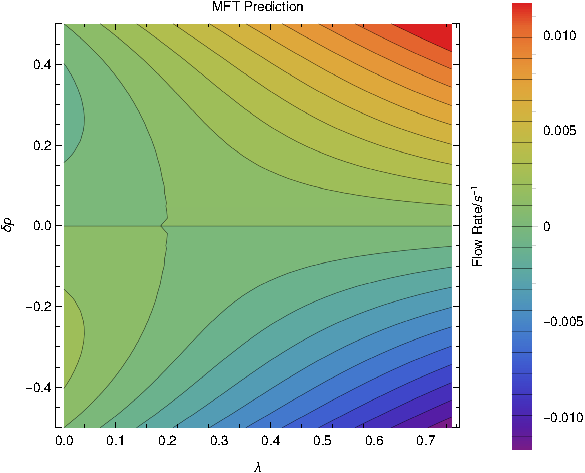
\includegraphics[width=0.98\linewidth]{newMftPred} \\
    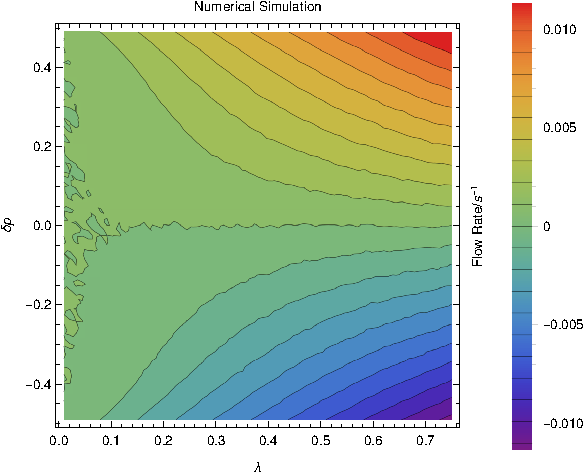
\includegraphics[width=0.98\linewidth]{newFlow}
    \end{tabular}
\end{center}
    \vspace{-2.5em}
\end{figure}


For relatively small driving force $\delta\rho$, we find
 $J$ varies approximately
linearly with $\delta\rho$, thus we can define 
$D_\mathrm{Eff}=\partDeriv{J}{\delta\rho}\big|_{\delta\rho=0}$, the effective diffusion coefficient and measure it using linear regression.
\begin{figure}[h!]
\vspace{1em}
\caption{\label{fig:diffCoef} Comparison of effective diffusion
  coefficient $D$ in the MFT (top) and in direct simulation (bottom)
  as a function of density and stickiness.  The region where MFT gives
  negative diffusion is represented as $D=0$. The simulations used 124
  sites averaged over $\sim 10^9$ steps at each of $12 \times 24
  \times 16 $ $(\lambda, \rho_M, \delta \rho)$ combinations.  Full
  details in the supplementary materials.}

\begin{center}
 \begin{tabular}{c}
    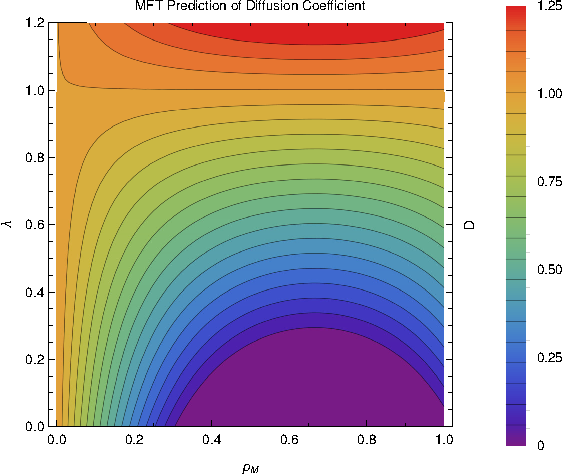
\includegraphics[width=0.98\linewidth]{newAnalFlow} \\
    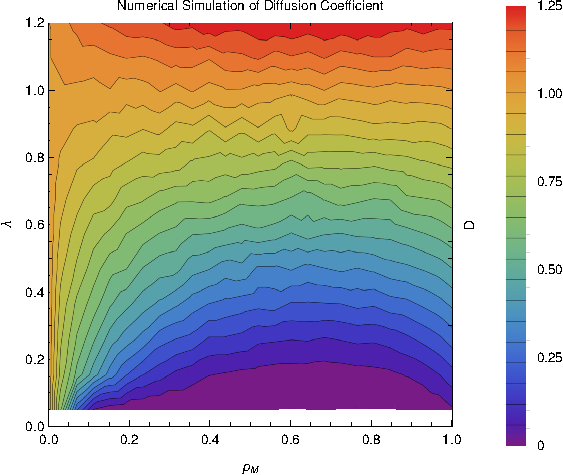
\includegraphics[width=0.98\linewidth]{newDataFlow}
    \end{tabular}
\end{center}
    \vspace{-2em}
\end{figure}

In Fig~\ref{fig:diffCoef} we compare the measured diffusion coefficient with the MFT result (Eq.~\ref{eq:MFTflow})
The MFT
and simulation agree well for low stickiness, and both show the 
maximum $D$ at $\rho_M = \frac{2}{3}$. For high stickiness, where the
MFT prediction gives a negative diffusion constant, measurement gives 
very low positive values for the current, making the determination of $D$ difficult; however, 
the important thing to note is that this critically slow flow corresponds to the
the negative-$D$ region predicted by the MFT (indicated in purple).

It is instructive to get an overview of how the SPM particles move
during flow. Fig.~\ref{fig:flowPatterns} shows a plot of the flow
structure in an interesting regime.  Over short timescales little
structure is visible, the dynamics appearing as a random walk with
some tendency for particles to clump; over longer timescales the
diffusive behavior is more evident, with a textured structure
suggesting characteristic velocity of particles or vacancies through
emergent correlated clumps.  In the limiting case of low $\lambda$ the
density of particles in the system tends to 1, irrespective of
boundary density: this may be because the interactions between
particles are strong enough that the filled state has lower chemical 
potential than either boundary.  Another interesting case is the limit of
high $\lambda$, where irrespective of boundary density, the internal
density tends to $\rho=\frac{2}{3}$, the value which gives maximal flow and maximum entropy production.  Additional plots can be found in the supplementary materials.

\begin{figure}[h!]
\caption{\label{fig:flowPatterns} Indicative spacetime flow pattern for sticky free-flow $\left[\lambda = \frac{3}{20}, (\rho_0, \rho_L) = (\frac{3}{4}, \frac{1}{4})\right]$; other combinations shown in the supplementary materials.
Time runs along the x-axis, space (1 pixel=1 site) along the y-axis, with grayscale tone (black being empty, white being full) illustrating average site occupation over (clockwise from top left) $\frac{1}{32}$, $1$, $8$ and $32$ Gillespie steps per site respectively.}
\begin{center}
 \begin{tabular}{c | c}
    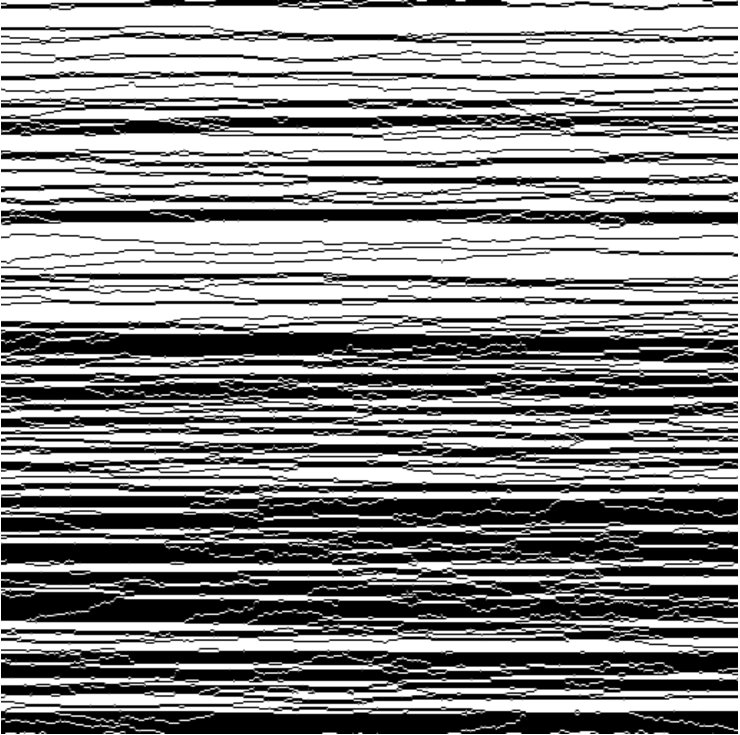
\includegraphics[width=0.49\linewidth]{shortTime}  &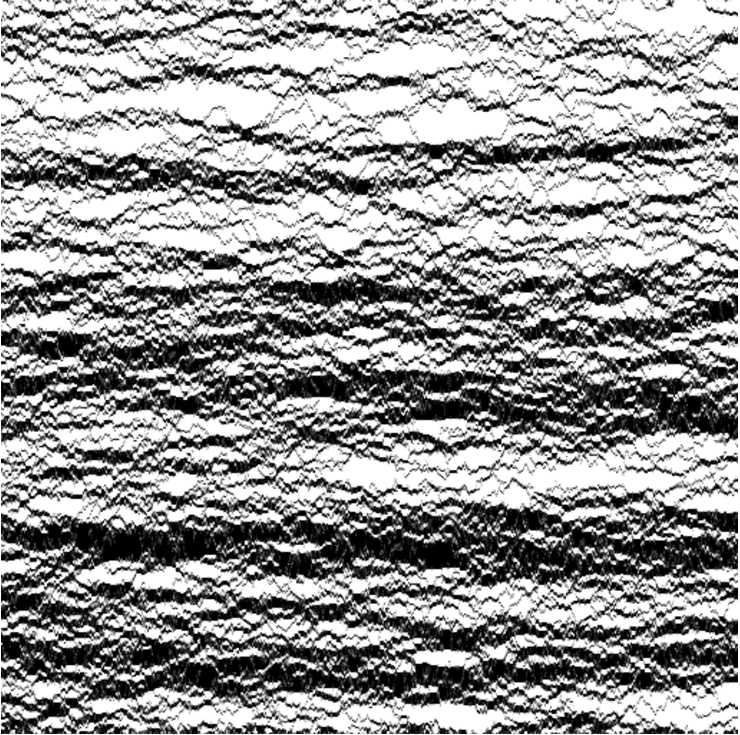
\includegraphics[width=0.49\linewidth]{midShortTime} \\
    \hline
    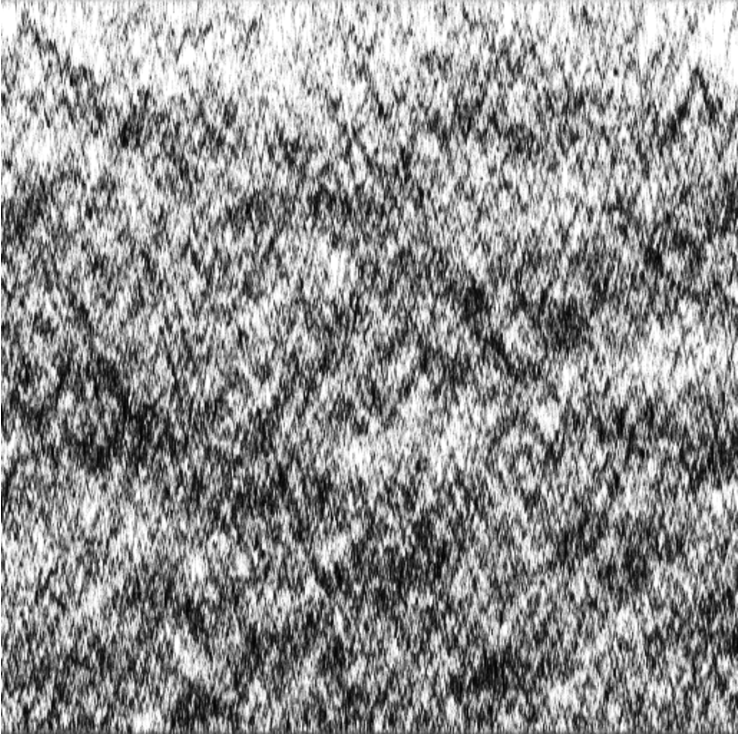
\includegraphics[width=0.49\linewidth]{longTime} &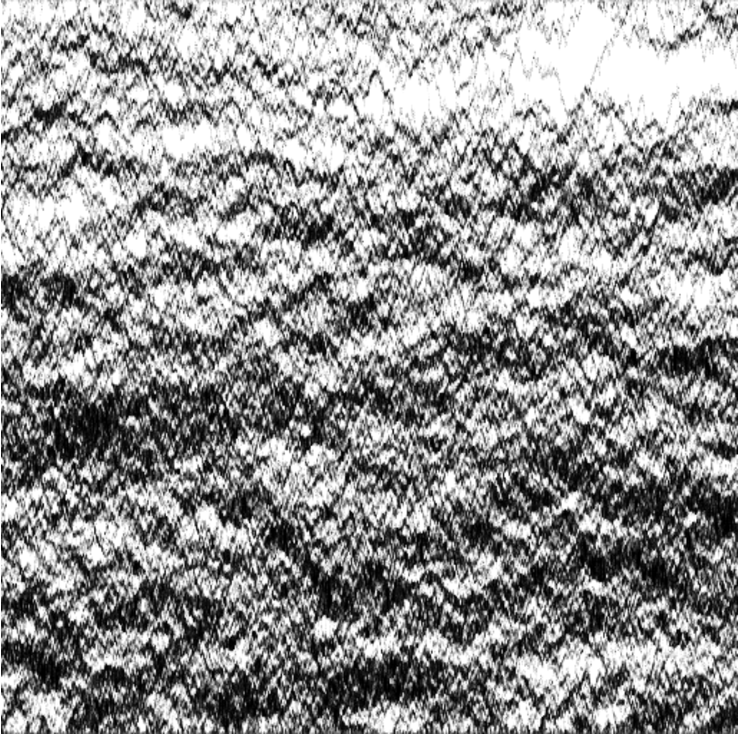
\includegraphics[width=0.49\linewidth]{midLongTime}
    \end{tabular}
\end{center}
    \vspace{-2em}
\end{figure}


To conclude, we have solved a nonlinear model for self-interacting sticky particles diffusing in 1D.  Although only the particles exhibit stickiness,  the analytics suggest a symmetry between vacancy-type and particle-type flow
at density of $\frac{2}{3}$, which is observed in the simulation.  The flow exhibits a foamy pattern with intermediate time-and-space correlations.  The continuum solution MFT is a good predictor of the bulk flow behavior of the SPM.
The negative diffusion constant found in MFT at high stickiness indicates  that the assumption of homogeneous density break down: thus the MFT predicts its own demise, and this agrees well with our numerics.

We would like to thank EPSRC (student grant 1527137) and Wolfson Foundation for providing the funding, Mikael Leetmaa for producing \texttt{KMCLib}, and the \texttt{Eddie3} team here at Edinburgh for maintaining the hardware used.
We would also like to thank Martin Evans, Bartek Waclaw and Richard Blythe for some very helpful discussions during the production of this letter.

%\bibliography{jHellStickyParticleMain.bib}

\begin{thebibliography}{33}%
\makeatletter
\providecommand \@ifxundefined [1]{%
 \@ifx{#1\undefined}
}%
\providecommand \@ifnum [1]{%
 \ifnum #1\expandafter \@firstoftwo
 \else \expandafter \@secondoftwo
 \fi
}%
\providecommand \@ifx [1]{%
 \ifx #1\expandafter \@firstoftwo
 \else \expandafter \@secondoftwo
 \fi
}%
\providecommand \natexlab [1]{#1}%
\providecommand \enquote  [1]{``#1''}%
\providecommand \bibnamefont  [1]{#1}%
\providecommand \bibfnamefont [1]{#1}%
\providecommand \citenamefont [1]{#1}%
\providecommand \href@noop [0]{\@secondoftwo}%
\providecommand \href [0]{\begingroup \@sanitize@url \@href}%
\providecommand \@href[1]{\@@startlink{#1}\@@href}%
\providecommand \@@href[1]{\endgroup#1\@@endlink}%
\providecommand \@sanitize@url [0]{\catcode `\\12\catcode `\$12\catcode
  `\&12\catcode `\#12\catcode `\^12\catcode `\_12\catcode `\%12\relax}%
\providecommand \@@startlink[1]{}%
\providecommand \@@endlink[0]{}%
\providecommand \url  [0]{\begingroup\@sanitize@url \@url }%
\providecommand \@url [1]{\endgroup\@href {#1}{\urlprefix }}%
\providecommand \urlprefix  [0]{URL }%
\providecommand \Eprint [0]{\href }%
\providecommand \doibase [0]{http://dx.doi.org/}%
\providecommand \selectlanguage [0]{\@gobble}%
\providecommand \bibinfo  [0]{\@secondoftwo}%
\providecommand \bibfield  [0]{\@secondoftwo}%
\providecommand \translation [1]{[#1]}%
\providecommand \BibitemOpen [0]{}%
\providecommand \bibitemStop [0]{}%
\providecommand \bibitemNoStop [0]{.\EOS\space}%
\providecommand \EOS [0]{\spacefactor3000\relax}%
\providecommand \BibitemShut  [1]{\csname bibitem#1\endcsname}%
\let\auto@bib@innerbib\@empty
%</preamble>
\bibitem [{\citenamefont {Belitsky}\ and\ \citenamefont
  {Sch{\"u}tz}(2011)}]{1742-5468-2011-07-P07007}%
  \BibitemOpen
  \bibfield  {author} {\bibinfo {author} {\bibfnamefont {V.}~\bibnamefont
  {Belitsky}}\ and\ \bibinfo {author} {\bibfnamefont {G.~M.}\ \bibnamefont
  {Sch{\"u}tz}},\ }\href {http://stacks.iop.org/1742-5468/2011/i=07/a=P07007}
  {\bibfield  {journal} {\bibinfo  {journal} {Journal of Statistical Mechanics:
  Theory and Experiment}\ }\textbf {\bibinfo {volume} {2011}},\ \bibinfo
  {pages} {P07007} (\bibinfo {year} {2011})}\BibitemShut {NoStop}%
\bibitem [{\citenamefont {Mobilia}\ \emph {et~al.}(2007)\citenamefont
  {Mobilia}, \citenamefont {Georgiev},\ and\ \citenamefont
  {T{\"a}uber}}]{Mobilia2007}%
  \BibitemOpen
  \bibfield  {author} {\bibinfo {author} {\bibfnamefont {M.}~\bibnamefont
  {Mobilia}}, \bibinfo {author} {\bibfnamefont {I.~T.}\ \bibnamefont
  {Georgiev}}, \ and\ \bibinfo {author} {\bibfnamefont {U.~C.}\ \bibnamefont
  {T{\"a}uber}},\ }\href {\doibase 10.1007/s10955-006-9146-3} {\bibfield
  {journal} {\bibinfo  {journal} {Journal of Statistical Physics}\ }\textbf
  {\bibinfo {volume} {128}},\ \bibinfo {pages} {447} (\bibinfo {year}
  {2007})}\BibitemShut {NoStop}%
\bibitem [{\citenamefont {Tegner}\ \emph {et~al.}(2015)\citenamefont {Tegner},
  \citenamefont {Zhu}, \citenamefont {Siemers}, \citenamefont {Saksl},\ and\
  \citenamefont {Ackland}}]{tegner2015high}%
  \BibitemOpen
  \bibfield  {author} {\bibinfo {author} {\bibfnamefont {B.}~\bibnamefont
  {Tegner}}, \bibinfo {author} {\bibfnamefont {L.}~\bibnamefont {Zhu}},
  \bibinfo {author} {\bibfnamefont {C.}~\bibnamefont {Siemers}}, \bibinfo
  {author} {\bibfnamefont {K.}~\bibnamefont {Saksl}}, \ and\ \bibinfo {author}
  {\bibfnamefont {G.}~\bibnamefont {Ackland}},\ }\href {\doibase
  10.1016/j.jallcom.2015.04.115} {\bibfield  {journal} {\bibinfo  {journal}
  {Journal of alloys and compounds}\ }\textbf {\bibinfo {volume} {643}},\
  \bibinfo {pages} {100} (\bibinfo {year} {2015})}\BibitemShut {NoStop}%
\bibitem [{\citenamefont {Zhu}\ \emph {et~al.}(2012)\citenamefont {Zhu},
  \citenamefont {Hu}, \citenamefont {Yang},\ and\ \citenamefont
  {Ackland}}]{zhu2012atomic}%
  \BibitemOpen
  \bibfield  {author} {\bibinfo {author} {\bibfnamefont {L.}~\bibnamefont
  {Zhu}}, \bibinfo {author} {\bibfnamefont {Q.-M.}\ \bibnamefont {Hu}},
  \bibinfo {author} {\bibfnamefont {R.}~\bibnamefont {Yang}}, \ and\ \bibinfo
  {author} {\bibfnamefont {G.}~\bibnamefont {Ackland}},\ }\href {\doibase
  10.1021/jp309305n} {\bibfield  {journal} {\bibinfo  {journal} {Journal of
  Physical Chemistry C}\ }\textbf {\bibinfo {volume} {116}},\ \bibinfo {pages}
  {24201} (\bibinfo {year} {2012})}\BibitemShut {NoStop}%
\bibitem [{\citenamefont {Deal}\ and\ \citenamefont
  {Grove}(1965)}]{DealGrove1965}%
  \BibitemOpen
  \bibfield  {author} {\bibinfo {author} {\bibfnamefont {B.~E.}\ \bibnamefont
  {Deal}}\ and\ \bibinfo {author} {\bibfnamefont {A.~S.}\ \bibnamefont
  {Grove}},\ }\href {\doibase 10.1063/1.1713945} {\bibfield  {journal}
  {\bibinfo  {journal} {Journal of Applied Physics}\ }\textbf {\bibinfo
  {volume} {36}},\ \bibinfo {pages} {3770} (\bibinfo {year} {1965})},\ \Eprint
  {http://arxiv.org/abs/https://doi.org/10.1063/1.1713945}
  {https://doi.org/10.1063/1.1713945} \BibitemShut {NoStop}%
\bibitem [{\citenamefont {Cabrera}\ and\ \citenamefont
  {Mott}(1949)}]{MottCabrera1949}%
  \BibitemOpen
  \bibfield  {author} {\bibinfo {author} {\bibfnamefont {N.}~\bibnamefont
  {Cabrera}}\ and\ \bibinfo {author} {\bibfnamefont {N.~F.}\ \bibnamefont
  {Mott}},\ }\href {http://stacks.iop.org/0034-4885/12/i=1/a=308} {\bibfield
  {journal} {\bibinfo  {journal} {Reports on Progress in Physics}\ }\textbf
  {\bibinfo {volume} {12}},\ \bibinfo {pages} {163} (\bibinfo {year}
  {1949})}\BibitemShut {NoStop}%
\bibitem [{\citenamefont {Buzzaccaro}\ \emph {et~al.}(2007)\citenamefont
  {Buzzaccaro}, \citenamefont {Rusconi},\ and\ \citenamefont
  {Piazza}}]{Buzzaccaro2007}%
  \BibitemOpen
  \bibfield  {author} {\bibinfo {author} {\bibfnamefont {S.}~\bibnamefont
  {Buzzaccaro}}, \bibinfo {author} {\bibfnamefont {R.}~\bibnamefont {Rusconi}},
  \ and\ \bibinfo {author} {\bibfnamefont {R.}~\bibnamefont {Piazza}},\ }\href
  {\doibase 10.1103/PhysRevLett.99.098301} {\bibfield  {journal} {\bibinfo
  {journal} {Phys. Rev. Lett.}\ }\textbf {\bibinfo {volume} {99}},\ \bibinfo
  {pages} {098301} (\bibinfo {year} {2007})}\BibitemShut {NoStop}%
\bibitem [{\citenamefont {Ladd}\ \emph {et~al.}(1988)\citenamefont {Ladd},
  \citenamefont {Colvin},\ and\ \citenamefont {Frenkel}}]{ladd1988application}%
  \BibitemOpen
  \bibfield  {author} {\bibinfo {author} {\bibfnamefont {A.~J.~C.}\
  \bibnamefont {Ladd}}, \bibinfo {author} {\bibfnamefont {M.~E.}\ \bibnamefont
  {Colvin}}, \ and\ \bibinfo {author} {\bibfnamefont {D.}~\bibnamefont
  {Frenkel}},\ }\href {\doibase 10.1103/PhysRevLett.60.975} {\bibfield
  {journal} {\bibinfo  {journal} {Phys. Rev. Lett.}\ }\textbf {\bibinfo
  {volume} {60}},\ \bibinfo {pages} {975} (\bibinfo {year} {1988})}\BibitemShut
  {NoStop}%
\bibitem [{\citenamefont {Liggett}(1985)}]{liggett1985interacting}%
  \BibitemOpen
  \bibfield  {author} {\bibinfo {author} {\bibfnamefont {T.~M.}\ \bibnamefont
  {Liggett}},\ }\href@noop {} {\emph {\bibinfo {title} {Interacting particle
  systems}}}\ (\bibinfo  {publisher} {Springer-Verlag, Berlin},\ \bibinfo
  {year} {1985})\BibitemShut {NoStop}%
\bibitem [{\citenamefont {Ben-Naim}\ \emph {et~al.}(1999)\citenamefont
  {Ben-Naim}, \citenamefont {Chen}, \citenamefont {Doolen},\ and\ \citenamefont
  {Redner}}]{BenNaim1999}%
  \BibitemOpen
  \bibfield  {author} {\bibinfo {author} {\bibfnamefont {E.}~\bibnamefont
  {Ben-Naim}}, \bibinfo {author} {\bibfnamefont {S.~Y.}\ \bibnamefont {Chen}},
  \bibinfo {author} {\bibfnamefont {G.~D.}\ \bibnamefont {Doolen}}, \ and\
  \bibinfo {author} {\bibfnamefont {S.}~\bibnamefont {Redner}},\ }\href
  {\doibase 10.1103/PhysRevLett.83.4069} {\bibfield  {journal} {\bibinfo
  {journal} {Phys. Rev. Lett.}\ }\textbf {\bibinfo {volume} {83}},\ \bibinfo
  {pages} {4069} (\bibinfo {year} {1999})}\BibitemShut {NoStop}%
\bibitem [{\citenamefont {Shandarin}\ and\ \citenamefont
  {Zeldovich}(1989)}]{Shandarin1989}%
  \BibitemOpen
  \bibfield  {author} {\bibinfo {author} {\bibfnamefont {S.~F.}\ \bibnamefont
  {Shandarin}}\ and\ \bibinfo {author} {\bibfnamefont {Y.~B.}\ \bibnamefont
  {Zeldovich}},\ }\href {\doibase 10.1103/RevModPhys.61.185} {\bibfield
  {journal} {\bibinfo  {journal} {Rev. Mod. Phys.}\ }\textbf {\bibinfo {volume}
  {61}},\ \bibinfo {pages} {185} (\bibinfo {year} {1989})}\BibitemShut
  {NoStop}%
\bibitem [{\citenamefont {Frachebourg}(1999)}]{Frachebourg1999}%
  \BibitemOpen
  \bibfield  {author} {\bibinfo {author} {\bibfnamefont {L.}~\bibnamefont
  {Frachebourg}},\ }\href {\doibase 10.1103/PhysRevLett.82.1502} {\bibfield
  {journal} {\bibinfo  {journal} {Phys. Rev. Lett.}\ }\textbf {\bibinfo
  {volume} {82}},\ \bibinfo {pages} {1502} (\bibinfo {year}
  {1999})}\BibitemShut {NoStop}%
\bibitem [{\citenamefont {{Frachebourg}}\ \emph {et~al.}(2000)\citenamefont
  {{Frachebourg}}, \citenamefont {{Martin}},\ and\ \citenamefont
  {{Piasecki}}}]{Frachebourg2000}%
  \BibitemOpen
  \bibfield  {author} {\bibinfo {author} {\bibfnamefont {L.}~\bibnamefont
  {{Frachebourg}}}, \bibinfo {author} {\bibfnamefont {P.~A.}\ \bibnamefont
  {{Martin}}}, \ and\ \bibinfo {author} {\bibfnamefont {J.}~\bibnamefont
  {{Piasecki}}},\ }\href {\doibase 10.1016/S0378-4371(99)00585-3} {\bibfield
  {journal} {\bibinfo  {journal} {Physica A Statistical Mechanics and its
  Applications}\ }\textbf {\bibinfo {volume} {279}},\ \bibinfo {pages} {69}
  (\bibinfo {year} {2000})},\ \Eprint {http://arxiv.org/abs/cond-mat/9911346}
  {cond-mat/9911346} \BibitemShut {NoStop}%
\bibitem [{\citenamefont {Obukhovsky}\ \emph {et~al.}(2017)\citenamefont
  {Obukhovsky}, \citenamefont {Kutsyk}, \citenamefont {Nikonova},\ and\
  \citenamefont {Ilchenko}}]{Obukhovsky2017}%
  \BibitemOpen
  \bibfield  {author} {\bibinfo {author} {\bibfnamefont {V.~V.}\ \bibnamefont
  {Obukhovsky}}, \bibinfo {author} {\bibfnamefont {A.~M.}\ \bibnamefont
  {Kutsyk}}, \bibinfo {author} {\bibfnamefont {V.~V.}\ \bibnamefont
  {Nikonova}}, \ and\ \bibinfo {author} {\bibfnamefont {O.~O.}\ \bibnamefont
  {Ilchenko}},\ }\href {\doibase 10.1103/PhysRevE.95.022133} {\bibfield
  {journal} {\bibinfo  {journal} {Phys. Rev. E}\ }\textbf {\bibinfo {volume}
  {95}},\ \bibinfo {pages} {022133} (\bibinfo {year} {2017})}\BibitemShut
  {NoStop}%
\bibitem [{\citenamefont {Gorokhova}\ and\ \citenamefont
  {Melnik}(2010)}]{Gorokhova2010}%
  \BibitemOpen
  \bibfield  {author} {\bibinfo {author} {\bibfnamefont {N.~V.}\ \bibnamefont
  {Gorokhova}}\ and\ \bibinfo {author} {\bibfnamefont {O.~E.}\ \bibnamefont
  {Melnik}},\ }\href {\doibase 10.1134/S0015462810050017} {\bibfield  {journal}
  {\bibinfo  {journal} {Fluid Dynamics}\ }\textbf {\bibinfo {volume} {45}},\
  \bibinfo {pages} {679} (\bibinfo {year} {2010})}\BibitemShut {NoStop}%
\bibitem [{\citenamefont {Sugden}\ and\ \citenamefont
  {Evans}(2007)}]{sugden2007dynamically}%
  \BibitemOpen
  \bibfield  {author} {\bibinfo {author} {\bibfnamefont {K.~E.~P.}\
  \bibnamefont {Sugden}}\ and\ \bibinfo {author} {\bibfnamefont {M.~R.}\
  \bibnamefont {Evans}},\ }\href
  {http://stacks.iop.org/1742-5468/2007/i=11/a=P11013} {\bibfield  {journal}
  {\bibinfo  {journal} {Journal of Statistical Mechanics: Theory and
  Experiment}\ }\textbf {\bibinfo {volume} {2007}},\ \bibinfo {pages} {P11013}
  (\bibinfo {year} {2007})}\BibitemShut {NoStop}%
\bibitem [{\citenamefont {Kollmann}(2003)}]{Kollmann2003}%
  \BibitemOpen
  \bibfield  {author} {\bibinfo {author} {\bibfnamefont {M.}~\bibnamefont
  {Kollmann}},\ }\href {\doibase 10.1103/PhysRevLett.90.180602} {\bibfield
  {journal} {\bibinfo  {journal} {Phys. Rev. Lett.}\ }\textbf {\bibinfo
  {volume} {90}},\ \bibinfo {pages} {180602} (\bibinfo {year}
  {2003})}\BibitemShut {NoStop}%
\bibitem [{\citenamefont {Lin}\ \emph {et~al.}(2005)\citenamefont {Lin},
  \citenamefont {Meron}, \citenamefont {Cui}, \citenamefont {Rice},\ and\
  \citenamefont {Diamant}}]{Lin2005}%
  \BibitemOpen
  \bibfield  {author} {\bibinfo {author} {\bibfnamefont {B.}~\bibnamefont
  {Lin}}, \bibinfo {author} {\bibfnamefont {M.}~\bibnamefont {Meron}}, \bibinfo
  {author} {\bibfnamefont {B.}~\bibnamefont {Cui}}, \bibinfo {author}
  {\bibfnamefont {S.~A.}\ \bibnamefont {Rice}}, \ and\ \bibinfo {author}
  {\bibfnamefont {H.}~\bibnamefont {Diamant}},\ }\href {\doibase
  10.1103/PhysRevLett.94.216001} {\bibfield  {journal} {\bibinfo  {journal}
  {Phys. Rev. Lett.}\ }\textbf {\bibinfo {volume} {94}},\ \bibinfo {pages}
  {216001} (\bibinfo {year} {2005})}\BibitemShut {NoStop}%
\bibitem [{\citenamefont {Hegde}\ \emph {et~al.}(2014)\citenamefont {Hegde},
  \citenamefont {Sabhapandit},\ and\ \citenamefont {Dhar}}]{Hegde2014}%
  \BibitemOpen
  \bibfield  {author} {\bibinfo {author} {\bibfnamefont {C.}~\bibnamefont
  {Hegde}}, \bibinfo {author} {\bibfnamefont {S.}~\bibnamefont {Sabhapandit}},
  \ and\ \bibinfo {author} {\bibfnamefont {A.}~\bibnamefont {Dhar}},\ }\href
  {\doibase 10.1103/PhysRevLett.113.120601} {\bibfield  {journal} {\bibinfo
  {journal} {Phys. Rev. Lett.}\ }\textbf {\bibinfo {volume} {113}},\ \bibinfo
  {pages} {120601} (\bibinfo {year} {2014})}\BibitemShut {NoStop}%
\bibitem [{\citenamefont {Krapivsky}\ \emph {et~al.}(2014)\citenamefont
  {Krapivsky}, \citenamefont {Mallick},\ and\ \citenamefont
  {Sadhu}}]{Krapivsky2014}%
  \BibitemOpen
  \bibfield  {author} {\bibinfo {author} {\bibfnamefont {P.~L.}\ \bibnamefont
  {Krapivsky}}, \bibinfo {author} {\bibfnamefont {K.}~\bibnamefont {Mallick}},
  \ and\ \bibinfo {author} {\bibfnamefont {T.}~\bibnamefont {Sadhu}},\ }\href
  {\doibase 10.1103/PhysRevLett.113.078101} {\bibfield  {journal} {\bibinfo
  {journal} {Phys. Rev. Lett.}\ }\textbf {\bibinfo {volume} {113}},\ \bibinfo
  {pages} {078101} (\bibinfo {year} {2014})}\BibitemShut {NoStop}%
\bibitem [{\citenamefont {Imamura}\ \emph {et~al.}(2017)\citenamefont
  {Imamura}, \citenamefont {Mallick},\ and\ \citenamefont
  {Sasamoto}}]{Imamura2017}%
  \BibitemOpen
  \bibfield  {author} {\bibinfo {author} {\bibfnamefont {T.}~\bibnamefont
  {Imamura}}, \bibinfo {author} {\bibfnamefont {K.}~\bibnamefont {Mallick}}, \
  and\ \bibinfo {author} {\bibfnamefont {T.}~\bibnamefont {Sasamoto}},\ }\href
  {\doibase 10.1103/PhysRevLett.118.160601} {\bibfield  {journal} {\bibinfo
  {journal} {Phys. Rev. Lett.}\ }\textbf {\bibinfo {volume} {118}},\ \bibinfo
  {pages} {160601} (\bibinfo {year} {2017})}\BibitemShut {NoStop}%
\bibitem [{\citenamefont {Kardar}\ \emph {et~al.}(1986)\citenamefont {Kardar},
  \citenamefont {Parisi},\ and\ \citenamefont {Zhang}}]{PhysRevLett.56.889}%
  \BibitemOpen
  \bibfield  {author} {\bibinfo {author} {\bibfnamefont {M.}~\bibnamefont
  {Kardar}}, \bibinfo {author} {\bibfnamefont {G.}~\bibnamefont {Parisi}}, \
  and\ \bibinfo {author} {\bibfnamefont {Y.-C.}\ \bibnamefont {Zhang}},\ }\href
  {\doibase 10.1103/PhysRevLett.56.889} {\bibfield  {journal} {\bibinfo
  {journal} {Phys. Rev. Lett.}\ }\textbf {\bibinfo {volume} {56}},\ \bibinfo
  {pages} {889} (\bibinfo {year} {1986})}\BibitemShut {NoStop}%
\bibitem [{\citenamefont {Krug}\ and\ \citenamefont
  {Spohn}(1988)}]{PhysRevA.38.4271}%
  \BibitemOpen
  \bibfield  {author} {\bibinfo {author} {\bibfnamefont {J.}~\bibnamefont
  {Krug}}\ and\ \bibinfo {author} {\bibfnamefont {H.}~\bibnamefont {Spohn}},\
  }\href {\doibase 10.1103/PhysRevA.38.4271} {\bibfield  {journal} {\bibinfo
  {journal} {Phys. Rev. A}\ }\textbf {\bibinfo {volume} {38}},\ \bibinfo
  {pages} {4271} (\bibinfo {year} {1988})}\BibitemShut {NoStop}%
\bibitem [{\citenamefont {Sasamoto}\ and\ \citenamefont
  {Spohn}(2010)}]{Sasamoto2010}%
  \BibitemOpen
  \bibfield  {author} {\bibinfo {author} {\bibfnamefont {T.}~\bibnamefont
  {Sasamoto}}\ and\ \bibinfo {author} {\bibfnamefont {H.}~\bibnamefont
  {Spohn}},\ }\href {\doibase 10.1103/PhysRevLett.104.230602} {\bibfield
  {journal} {\bibinfo  {journal} {Phys. Rev. Lett.}\ }\textbf {\bibinfo
  {volume} {104}},\ \bibinfo {pages} {230602} (\bibinfo {year}
  {2010})}\BibitemShut {NoStop}%
\bibitem [{\citenamefont {Kawasaki}(1966)}]{PhysRev.145.224}%
  \BibitemOpen
  \bibfield  {author} {\bibinfo {author} {\bibfnamefont {K.}~\bibnamefont
  {Kawasaki}},\ }\href {\doibase 10.1103/PhysRev.145.224} {\bibfield  {journal}
  {\bibinfo  {journal} {Phys. Rev.}\ }\textbf {\bibinfo {volume} {145}},\
  \bibinfo {pages} {224} (\bibinfo {year} {1966})}\BibitemShut {NoStop}%
\bibitem [{\citenamefont {Katz}\ \emph {et~al.}(1984)\citenamefont {Katz},
  \citenamefont {Lebowitz},\ and\ \citenamefont {Spohn}}]{Katz1984}%
  \BibitemOpen
  \bibfield  {author} {\bibinfo {author} {\bibfnamefont {S.}~\bibnamefont
  {Katz}}, \bibinfo {author} {\bibfnamefont {J.~L.}\ \bibnamefont {Lebowitz}},
  \ and\ \bibinfo {author} {\bibfnamefont {H.}~\bibnamefont {Spohn}},\ }\href
  {\doibase 10.1007/BF01018556} {\bibfield  {journal} {\bibinfo  {journal}
  {Journal of Statistical Physics}\ }\textbf {\bibinfo {volume} {34}},\
  \bibinfo {pages} {497} (\bibinfo {year} {1984})}\BibitemShut {NoStop}%
\bibitem [{\citenamefont {Zia}(2010)}]{Zia2010}%
  \BibitemOpen
  \bibfield  {author} {\bibinfo {author} {\bibfnamefont {R.~K.~P.}\
  \bibnamefont {Zia}},\ }\href {\doibase 10.1007/s10955-009-9884-0} {\bibfield
  {journal} {\bibinfo  {journal} {Journal of Statistical Physics}\ }\textbf
  {\bibinfo {volume} {138}},\ \bibinfo {pages} {20} (\bibinfo {year}
  {2010})}\BibitemShut {NoStop}%
\bibitem [{\citenamefont {Kafri}\ \emph {et~al.}(2003)\citenamefont {Kafri},
  \citenamefont {Levine}, \citenamefont {Mukamel}, \citenamefont {Sch\"utz},\
  and\ \citenamefont {Willmann}}]{Kafri2003}%
  \BibitemOpen
  \bibfield  {author} {\bibinfo {author} {\bibfnamefont {Y.}~\bibnamefont
  {Kafri}}, \bibinfo {author} {\bibfnamefont {E.}~\bibnamefont {Levine}},
  \bibinfo {author} {\bibfnamefont {D.}~\bibnamefont {Mukamel}}, \bibinfo
  {author} {\bibfnamefont {G.~M.}\ \bibnamefont {Sch\"utz}}, \ and\ \bibinfo
  {author} {\bibfnamefont {R.~D.}\ \bibnamefont {Willmann}},\ }\href {\doibase
  10.1103/PhysRevE.68.035101} {\bibfield  {journal} {\bibinfo  {journal} {Phys.
  Rev. E}\ }\textbf {\bibinfo {volume} {68}},\ \bibinfo {pages} {035101}
  (\bibinfo {year} {2003})}\BibitemShut {NoStop}%
\bibitem [{\citenamefont {Gillespie}(1977)}]{Gillespie1977}%
  \BibitemOpen
  \bibfield  {author} {\bibinfo {author} {\bibfnamefont {D.~T.}\ \bibnamefont
  {Gillespie}},\ }\href {\doibase 10.1021/j100540a008} {\bibfield  {journal}
  {\bibinfo  {journal} {The Journal of Physical Chemistry}\ }\textbf {\bibinfo
  {volume} {81}},\ \bibinfo {pages} {2340} (\bibinfo {year} {1977})},\ \Eprint
  {http://arxiv.org/abs/http://dx.doi.org/10.1021/j100540a008}
  {http://dx.doi.org/10.1021/j100540a008} \BibitemShut {NoStop}%
\bibitem [{\citenamefont {Bortz}\ \emph {et~al.}(1975)\citenamefont {Bortz},
  \citenamefont {Kalos},\ and\ \citenamefont {Lebowitz}}]{Bortz1975}%
  \BibitemOpen
  \bibfield  {author} {\bibinfo {author} {\bibfnamefont {A.}~\bibnamefont
  {Bortz}}, \bibinfo {author} {\bibfnamefont {M.}~\bibnamefont {Kalos}}, \ and\
  \bibinfo {author} {\bibfnamefont {J.}~\bibnamefont {Lebowitz}},\ }\href
  {\doibase https://doi.org/10.1016/0021-9991(75)90060-1} {\bibfield  {journal}
  {\bibinfo  {journal} {Journal of Computational Physics}\ }\textbf {\bibinfo
  {volume} {17}},\ \bibinfo {pages} {10 } (\bibinfo {year} {1975})}\BibitemShut
  {NoStop}%
\bibitem [{\citenamefont {Prados}\ \emph {et~al.}(1997)\citenamefont {Prados},
  \citenamefont {Brey},\ and\ \citenamefont {S{\'a}nchez-Rey}}]{Prados1997}%
  \BibitemOpen
  \bibfield  {author} {\bibinfo {author} {\bibfnamefont {A.}~\bibnamefont
  {Prados}}, \bibinfo {author} {\bibfnamefont {J.~J.}\ \bibnamefont {Brey}}, \
  and\ \bibinfo {author} {\bibfnamefont {B.}~\bibnamefont {S{\'a}nchez-Rey}},\
  }\href {\doibase 10.1007/BF02765541} {\bibfield  {journal} {\bibinfo
  {journal} {Journal of Statistical Physics}\ }\textbf {\bibinfo {volume}
  {89}},\ \bibinfo {pages} {709} (\bibinfo {year} {1997})}\BibitemShut
  {NoStop}%
\bibitem [{\citenamefont {{Leetmaa}}\ and\ \citenamefont
  {{Skorodumova}}(2014)}]{leetmaa2014kmclib}%
  \BibitemOpen
  \bibfield  {author} {\bibinfo {author} {\bibfnamefont {M.}~\bibnamefont
  {{Leetmaa}}}\ and\ \bibinfo {author} {\bibfnamefont {N.~V.}\ \bibnamefont
  {{Skorodumova}}},\ }\href {\doibase 10.1016/j.cpc.2014.04.017} {\bibfield
  {journal} {\bibinfo  {journal} {Computer Physics Communications}\ }\textbf
  {\bibinfo {volume} {185}},\ \bibinfo {pages} {2340} (\bibinfo {year}
  {2014})},\ \Eprint {http://arxiv.org/abs/1405.1221} {arXiv:1405.1221
  [physics.comp-ph]} \BibitemShut {NoStop}%
\bibitem [{\citenamefont {Hellier}(2018)}]{jHellGitRepo}%
  \BibitemOpen
  \bibfield  {author} {\bibinfo {author} {\bibfnamefont {J.}~\bibnamefont
  {Hellier}},\ }\href {\doibase 10.5281/zenodo.1162818} {\  (\bibinfo {year}
  {2018}),\ 10.5281/zenodo.1162818}\BibitemShut {NoStop}%
\end{thebibliography}

\newpage


\end{document}
%
% ****** End of file apssamp.tex ******
